\documentclass[a4paper,12pt]{article} %размер бумаги устанавливаем А4, шрифт 12пунктов
\usepackage[T2A]{fontenc}
\usepackage[utf8]{inputenc}	%кодировка
\usepackage[english, russian]{babel}%используем русский и английский языки с переносами
\usepackage{amssymb, amsfonts, amsmath, cite, enumerate, float, indentfirst} %пакеты расширений
\usepackage{graphicx}
\usepackage{alltt}
%\usepackage[dvips]{graphicx} %вставка графики
\graphicspath{{images/}}%путь к рисункам
%%% Дополнительная работа с математикой
\usepackage{amsmath,amsfonts,amssymb,amsthm,mathtools} % AMS
\usepackage{icomma} % "Умная" запятая: $0,2$ --- число, $0, 2$ --- перечисление
\mathtoolsset{showonlyrefs=true} % Показывать номера только у тех формул, на которые есть \eqref{} в тексте.


% в преамбуле
\usepackage{longtable} 
\usepackage{array}

\renewcommand{\arraystretch}{1.5} % циферкой регулируется высота

\makeatletter
\renewcommand{\@biblabel}[1]{#1.} % Заменяем библиографию с квадратных скобок на точку:
\makeatother

\usepackage{geometry} % Меняем поля страницы
\geometry{left=2cm}% левое поле
\geometry{right=1.5cm}% правое поле
\geometry{top=1cm}% верхнее поле
\geometry{bottom=2cm}% нижнее поле

\begin{document}
РАЗРАБОТКА ИНФРАСТРУКТУРЫ АВТОМАТИЧЕСКОГО РАЗВЕРТЫВАНИЯ, ТЕСТИРОВАНИЯ И ОБСЛУЖИВАНИЯ СЕРВЕРНЫХ КОМПОНЕНТОВ ИНФОРМАЦИОННЫХ СИСТЕМ
\tableofcontents
\newpage
\section{Введение}
В настоящее время все чаще внедряются сложные механизмы для облегчения различных процессов проектирования и производства в компаниях различного масштаба. Из-за достижения высоких технологий в различных областях промышленности очень сильно возросли требования к программному продукту. В связи с этим, реализация программ стала гораздо сложнее и требует больших усилий. 

Создавая программный продукт, работающий на удаленном компьютере - сервере и взаимодействующий с множеством клиентов, необходимо использовать множество средств, помогающих реализовывать, поддерживать и развивать разрабатываемый продукт. Из таких средств можно выделить различного рода программные библиотеки, программные и виртуальные среды, набор утилит для нужд программной реализации, ее отладки, тестов и запуска приложения.

Во все времена первостепенным средством для разработки являлась компьютерная операционная система ОС. Именно она содержала минимальный набор средств для создания продукта. Таким образом, имея только консоль и даже консольный текстовый редактор, можно было создавать программы. 
Но с развитием технологий требования усложнялись, подходы программирования становились сложнее и эффективнее. В наши дни недостаточно "пустой" операционной системы, чтобы реализовать сложное приложение. Программы наделили сложным графическим интерфейсом, они стали способны работать удаленно и использовать общие пользовательские ресурсы вместо личный локальных.
Изменились и подходы к созданию таких приложений. Перед началом разработки необходимо оценить важность работы, назвать и рассмотреть основные стадии ее реализации от начала развития до внедрения. Сегодня проблемы развития продукта решают различные методологии и практики разработки софта. 
Среди них известны такие, как 
\begin{itemize}
\item Водопадная методика
\item Спиралевидная методика
\item Инкрементальная методика
\item V-Model 
\item Agile
\item и другие
\end{itemize}
Для всех методик можно назвать общие этапы разработки ПО, и как минимум это тестирование и внедрение продукта. Если в процессе написания кода и сборки проекта используются известные среды разработки, то при выполнении вышеупомянутых этапов может не существовать подходящего решения для быстрой отладки, проверки работоспособности написанной программеы вскупе с другими компонентами системы. В данном случае необходимо реализовать собственные решения для эффективного тестирования.
\newpage
\section{Модель}

\begin{quote}
\itshape{\large Мультитенантность} --- элемент архитектуры программного обеспечения, где единый экземпляр приложения, запущенного на сервере, обслуживает множество организаций-клиентов. Мультитенантность противопоставляется архитектуре из множественных экземпляров (англ. multiinstance), где для каждой организации-клиента создаются отдельные программные экземпляры. В мультиарендной архитектуре программные приложения работают одновременно с несколькими конфигурациями и наборами данных нескольких организаций, а каждая организация-клиент работает со своим экземпляром виртуального приложения, видя только свою конфигурацию и свой набор данных.
\end{quote}

%\begin{quote} Это абзац с отступами 1 см по бокам.
%    \begin{quote} А у этого отступы уже 2 см.
%    \end{quote}
%\end{quote}

%\rule{6cm}{0.4pt}\\[8pt]

\vspace{6pt}

\subsection{Схема инфраструктуры}
Для каждого разрабатываемого приложения известны сценарии его использвания и способы предоставления услуг. В данном случае, финальным результатом будет являться веб-приложение типа SaaS\footnote{%
	SaaS (англ. software as a service - программное обеспечение как услуга) --- одна из форм облачных вычислений, модель обслуживания, при которой подписчикам предоставляется готовое прикладное программное обеспечение, полностью обслуживаемое провайдером. Поставщик в этой модели самостоятельно управляет приложением, предоставляя заказчикам доступ к функциям с клиентских устройств, как правило через мобильное приложение или веб-браузер.
}. В качестве точки входа выступает сслыка в приложение для каждого клиента очередной организации. После этого каждому пользователю доступна площадка, в которой он может хранить различные файлы-модели, полученные в САПР приложениях, включая любую доументацию. На уровне организации доступна единая область памяти, способная быть ограниченной для любого члена организации. 

В итоге получаем информационную систему с возможностью изолированно обслуживать пользователей из разных организацией (т.е. независимых подписчиков SaaS) в рамках одного сервиса. Основным здесь является соблюдение изолированности подписчиков друг от друга. Действительно, клиенты не обрадуются, если данные, которые они хранят в SaaS приложении, будут доступны при поиске для других клиентов. Это явное нарушение изолированности.

Для реализации можно взять один сервер, одну операционную систему, одну базу данных. Механизм изоляции будет осуществляться с помощью особого хранения данных в таблицах БД и записью файлов в общую файловую сисему, а так же обработкой и перенаправлением web-запросов от клиентов на микросервисы.

Для достижения поставленных целей можно рассмотреть слудующую архитектуру сервера:

\begin{center}
	\begin{tabular}[t]{|c|p{15em}|}
		\hline
			ДНС-сервер\\
		\hline
			Прокси-сервер\\
		\hline
			Backend\\
		\hline
			БД\\
		\hline
			Файловое хранилище\\
		\hline
			Средства инфраструктуры\\
		\hline
	\end{tabular}
\end{center}

Каждый уровенень выполняет определенную роль. В совокупности c развитыми средствами автоматизации инфрастуктуры они реализуют целостную структуру информационной системы приложения. Далее будут рассмотрена каждый из них.

\subsection{Уровень ДНС-сервера}

\begin{quote}
\itshape{\large Доменное имя} --- основа для имени сайта, с помощью которой можно попасть на его ресурс.\\
\itshape{\large Доменная зона} --- совокупность доменных имён определённого уровня, входящих в конкретный домен.\\
\itshape{\large Делегирование} --- это передача контроля над частью доменной зоны другой ответственной стороне.
\end{quote}

\begin{figure}[H]
\centering
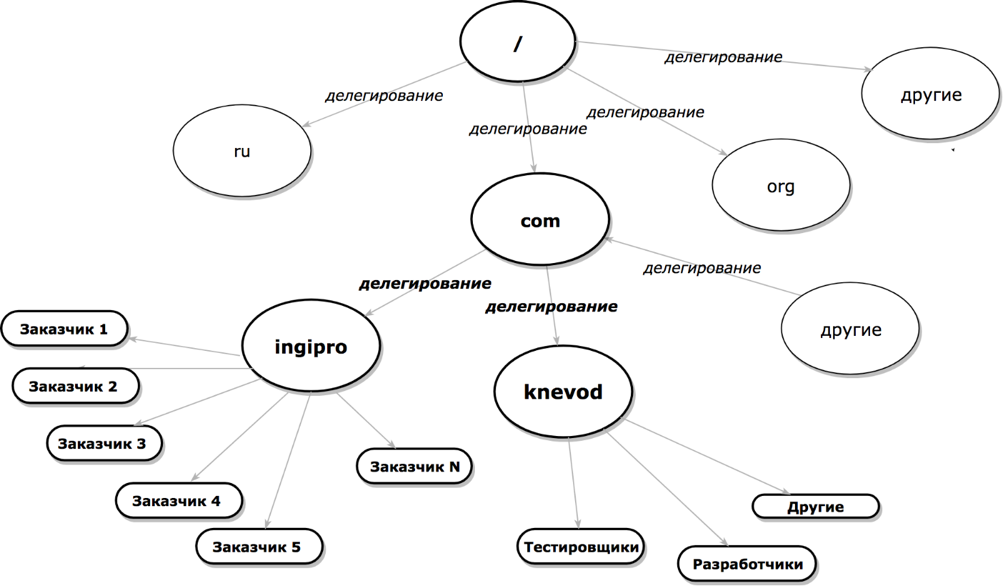
\includegraphics[scale=0.9]{dns.png}
\caption{Иерархия доменных имен}
\label{img:domains}
\end{figure}

ДНС\footnote{%
	DNS (англ. Domain Name System «система доменных имён») — компьютерная распределённая система для получения информации о доменах. Чаще всего используется для получения IP-адреса по имени хоста (компьютера или устройства), получения информации о маршрутизации почты, обслуживающих узлах для протоколов в домене.
} сервер в данной ситуации играет важную роль. На уровне доменных имен происходит разделенный досуп к инфрмационной системе. Это самый верхний уровень, который помогает реализовать множество точек входа в систему. Для того, чтобы добавить еще одного польователя, необходимо будет добавить в доменную зону новое имя, выделяемое для заказчика.

Так, например, если информационная система доступна по имени ingipro.com, то дабавив имя new-company в зону и получив адрес {\bfseries new-company.ingipro.com}, мы можем назначить клиенту этот адрес. Остальной механизм валидации осуществляется на следующих уровнях. 

В данном проекте используется Bind в качестве ДНС-сервера.

\subsection{Уровень Прокси-сервера}

На роль Прокси-сервера\footnote{%
	Прокси-сервер (от англ. proxy — «представитель», «уполномоченный») — промежуточный сервер в компьютерных сетях, выполняющий роль посредника между пользователем и целевым сервером, позволяющий клиентам как выполнять косвенные запросы (принимая и передавая их через прокси-сервер) к другим сетевым службам, так и получать ответы.
} возлагается много задач. Среди них:
\begin{itemize}
\item Обработка запрашиваемого адреса с целью перенаправления на другой адрес
\item Фильтрация и перенаправление запросов на уровень Backend
\item Выдача специальных ресурсов для запрашиваемого доменного уровня
\item Выдача статических ресурсов на сторону клиента
\end{itemize}

На этом уровне Веб-сервер\footnote{%
	Веб-сервер --- сервер, принимающий HTTP-запросы от клиентов, обычно веб-браузеров, и выдающий им HTTP-ответы, как правило, вместе с HTML-страницей, изображением, файлом, медиа-потоком или другими данными.
} Nginx, выступающий в роли Прокси-сервера, принимает HTTP-запросы от клиентов, перенаправляет их на необходимые микросервисы, которые в свою очередь реализуют основную логику работы разрабатываемого приложения. Далее возвращает в ответ HTTP-ответ с необходимым содержимым для отображения графического дизайна и данных в браузере клиента.


\subsection{Уровень Backend}

Backend\footnote{Backend --- программно-аппаратная часть сервиса. Набор приложений сервиса, работающих на стороне сервера.} является основной логической частью веб-приложения. Его архитектура бывает монолитной и микросервисной. В текущем проекте реализуется микросервисная архитекрура, состоящая из отдельных приложений, выполняющих специальные задачи. Так, например, существует микросервис, отвечающий за авторизацию пользователя в системе; микросервис, отвечающий за передачу файловых данных клиенту; микросервис, в основную задачу которого входит хранение множества атрибутов клиента; микросервис, отвечающий за отрисовку графических данных и так далее\dots

Каждый микросервис работает на специально выделенном сетевом порту сервера. В зависимости от поступившего от клиента HTTP-запроса происходит перенаправление на конкретный микросервис через сетевой порт. Во время работы Backend оперирует базой даных и файлами, располагающихся на жестком диске. Так проиходит обмен между уровнями инфраструктуры.
 
\subsection{Уровень Базы данных}

Огромное количество информации пользователей хранится в базе данных. Для ее управления используется СУБД\footnote{СУБД --- Система управления базой данных} PostgreSQL. Через нее микросервисы получают данные пользователей, хранящиеся в таблицах. Для достижения принципа мультитенантности реализуется следующий подход: пусть выделенная экосистема для клинета, называется new-company (по имени домена). Экосистема\footnote{Изолированное информационное пространство клиента для работы с сервисами приложения. Любые данные хранимые в экосистеме, связаны только с ней и клиентом на всех уровнях модели сервера.} в БД представляется двумя таблицами {\ttfamily attr\_new-company}, {\ttfamily entity\_new-company} и одной последовательностью {\ttfamily entity\_seq\_new-company}. Каждая заводимая экосистема хранит три объекта базы данных, которые относятся только к ней. Таким образом изолируются данные клиентов на уровне БД.

\subsection{Уровень файлового хранилища}

Уровень файлового хранилища представляет из себя часть файловой системы, находящейся на локальном или удаленном диске. Тут хранятся гораздо более тяжелые данные мультимедийного характера: документы, изображения, чертежи, аудио и видео записи. Область файлового хранилища закрыта от системных пользователей на уровне ОС и доступ туда имеют только программы, относящиеся к сервису. Как было сказано выше, любые данные Экосистемы имеют отношение только к ней самой. Поэтому в способ хранения информации Экосистемы выглядит слудующим образом:
\begin{figure}[H]
%\centering
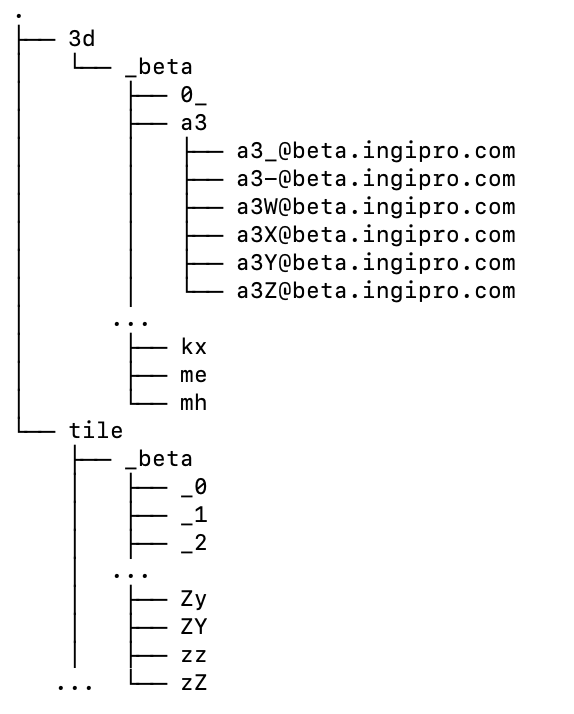
\includegraphics[scale=0.9]{tree.png}
\caption{Структура файлового хранилища}
\label{img:tree}
\end{figure}

На (рис. \ref{img:tree}) показан пример для экосистемы под названием {\ttfamily \_beta}. Таким структурированным образом хранится информация любых документов, изображений и моделей систем САПР в виде отдельных тайлов.

\subsection{Средства инфраструктуры}

Все вышеописанные уровни модели сервера реализуют определенные задачи. Все вместе они формируют программную систему, которая предлагается как конечный продукт. За реализацию каждого уровня отвечает определенный разрабочик или команда разработчиков. Они используют собственные средства, обычно не совместимые с продуктами других уровней. Это разные языки программирования, сетевые интерфейсты, логика работы приложения, конфигурационные файлы. Часто для внедрения новой версии, например backend, требуется внесения изменений в веб-сервере или DNS-сервере. Это несет некоторые трудности, так как требует работы нескольких команд или людей. 

Для решения подобных проблем выступают различные сервисы непреревной интеграции и доставки. Они оперируют специальными агентами, которые выполняют конкретные задачи при замене версий. Главной целью средств инфраструктуры выступает автоматизация процессов обновления, останова и запуска. Это всегда уникальные решения, которые адаптированы для текущей системы.
\newpage
\section{Автоматизация процессов}

\begin{quote}
\sffamily Под автоматизацией процессов будем понимать набор действий по сборке программного продукта (backend, frontend), действий по управлению  сервисами (останов, запуск, перезапуск), действий по работе с конфигурационными файлами используемых программ и действий по обновлению версий микросервисов, сайта и прочее.
\end{quote}


\subsection{Автоматизация сборки микросервисов}

Много действий по разработке ПО связано с постоянными изменениями в коде, его дополнении и тестировании. Поэтому очень часто приходится пересобирать из исходного кода часть программного продукта. Особенно часто обращает на себя внимаение Backend с его микросервисами. 

Для достижения цели конечного продукта используется 2 сервера: отладочный и производственный. Цели отладочного сводятся непосредственно к разработке ПО, ее отладке и тестированию. Финальную версию ПО выкладывают на производственный сервер, где клиенты пользуются сервисом, пока на отладочном происходит разработка новой версии программного продукта.

Ниже приводится автоматический алгоритм, используемый в текущем проекте:

\begin{enumerate}
	\item Проверка наличия и синтаксиса конфигурационного файла.
	\item Обновление Исходного кода из удаленного репозитория.
	\begin{enumerate}
		\item Проверка текущей ветки;
		\item Обновления копии локального репозитория из удаленной ветки.
	\end{enumerate}
	\item Обновление и модификация UPP\footnote{U ++ --- это кроссплатформенная среда быстрой разработки приложений на C ++, ориентированная на производительность труда программистов. Он включает в себя набор библиотек (GUI, SQL и т.д.) И интегрированную среду разработки.}.
	\begin{enumerate}
		\item Сброс локального репозитория до первоначального состояния;
		\item Обновление из официального репозитория;
		\item Наложение патчей, подготовленных программистами микросервисов в отдельной локальной ветке.
	\end{enumerate}
	\item Выполнение сборки микросервисов.
	\begin{enumerate}
		\item Проверка разрешения на пересборку конкретного микросервиса.
		\item Выполнение сборки проекта микросервиса с помощью встроенного во фреймворк UPP инструмента umk. При сборке указываются необходимые для сборки каждого микросервиса флаги и ключи сборки, конечный путь для новых собранных бинарных файлов.
		\item Установка метки статуса сборки в скрытый временный файл;
		\item Сохранение старой версии микросервиса в файл в постфиксом '.old' в директорию с микросервисом.
	\end{enumerate}
	\item Вызов модуля тестирования микросервисов
	\begin{enumerate}
		\item Проверка статуса сборки;
		\item Вызов модуля UNIT тестов;
		\item Вызов модуля регрессионного тестирования.
	\end{enumerate}
	\item Корректное завершение процессов.
	\begin{enumerate}
		\item Проверка статусов тестирования;
		\item Проверка разрешения на перезапуск микросервиса;
		\item Чтение из конфигурационного файла переменной, содержащей максимальное время ожидания программного завершения микросервиса;
		\item Отправка процессу программного сигнала завершения SIGINT и старт таймера;
		\item Ожидание завершения. Отправка SIGKILL, если процесс не успел завершиться за указанный интервал времени;
		\item Проверка закрытия сетевых портов;
		\item Установка метки статуса сокета, на котором работал микросервис;
	\end{enumerate}
	\item Запуск микросервисов и проверка их состояния.
	\begin{enumerate}
		\item Проверка статуса сетевого порта;
		\item Запуск и демонизация\footnote{Демонизацией процесса называют запуск программы для работы в специальном фоновом режиме даже если пользователь выйдет из системы.} микросервиса;
		\item Ожидание некоторого времени и проверка состояния процесса.
	\end{enumerate}
\end{enumerate}


\subsection{Автоматизация перезапуска микросервисов}

Для реализации перезапуска микросервисов потребовался отдельный скрипт, который отвечает за передачу сигнала прерывания в микросервис и обработку реакции останавливаемой программы на сигнал.
Общий алгоритм останова и перезапуска микросервиса в автоматическом режиме следующий:
\begin{enumerate}
 	\item Проверка разрешения на перезапуск, отмеченным в конфигурационном файле.
 	\item Проверка наличия рабочих процессов микросервиса в системе.
 	\item Отправка сигнала SIGINT на программное завершение.
 	\item Ожидание корректного завершения микросервиса и всех его дочерних процессов в течение указанного в конфигурационном файле времени. Если процесс не завершился самостоятельно, производится отправка сигнала принудительного завершения SIGKILL.
 	\item Ожидание закрытия сетевого порта микросервиса. Если порт не закрывается в течение указанного времени (10 секунд), то автосборка отражает это состояние в параметре статуса порта. 
 	\item Проверка состояние сетевого порта по флагу. Если порт не был закрыт, то процесс автосборки завершается с определенным кодом. 	
\end{enumerate}

Алгоритм ручного перезапуска вызывается в режиме '-restart' и аналогичен автоматическому. Алгоритмы останова и запуска требуют каждый проверку порта, для этого и введен параметр состояния порта. Это необходимо для гарантированного завершения микросервиса. 
Реализованный механизм останова и запуска микросервиса достаточно гибкий, так как включает в себя несколько проверок. Это позволяет максимально корректно завершить работу микросервиса, в каком бы он состоянии не находился.


\subsection{Автоматизация замены версии микросервисов}

Процесс замены версий на отладочном и производственном серверах отличается. Любая сборка проекта происходит на отладочном сервере. В данном случае, как и в случае с автоматизацией сборки и перезапуска микросервисов, учавствует специльно реализованная программа. На отладочном сервере для замены версии микросервисов можно воспользоваться этой утилитой для сборки. Так она перезапишет локальные версии программ. С производственным сервером немного сложнее, так как нужно локально собрать ПО и доставить его. Алгоритм можно описать так:
\begin{enumerate}
	\item Проверка наличия и синтаксиса конфигурационного файла автосборки
	\item Проверка существования бинарных файлов и формирование их списка
	\item Установление SSH соединения с боевым сервером
	\item Остановка микросервисов, используя тот же алгоритм автосборки
	\item Создание бэкапа каждого микросервиса
	\item Перезапись старых бинарных файлов новыми
	\item Запуск микросервисов
	\item Разрыв SSH соединения
\end{enumerate}
На производственном сервере существует две версии одновременно работающих Backend: Beta\footnote{Бета-версия продукта. Используется для предрелиза продукта. В очередной раз команда убеждается, что все работает корректно.} и Production\footnote{Конечый вариант продукта, доступный для использования клиентам.}. Рис. \ref{img:updating} показывает нагладное отношение объектов и последовательность обновления микросервисов.

\begin{figure}[H]
\centering
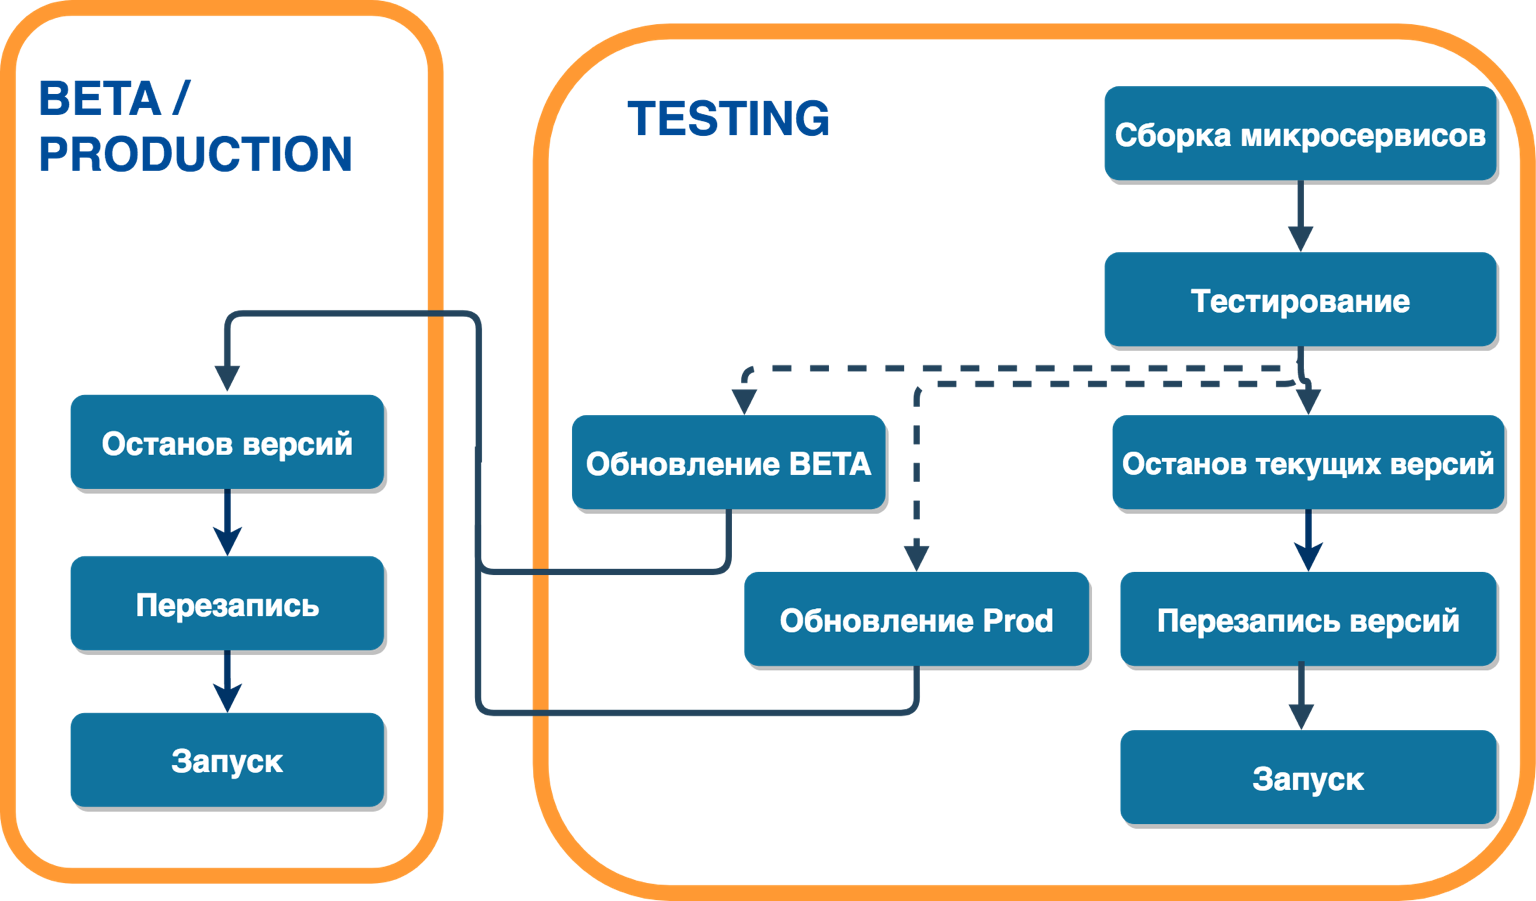
\includegraphics[scale=0.6]{updating.png}
\caption{Схема замены версий на серверах}
\label{img:updating}
\end{figure} 


\subsection{Автоматизация создания доменного имени}

Доменное имя - это самый высокоуровневый атрибут экосистемы клиента. Именно он является визуальной составляющей точки входа в систему, т.е. клиент его видет самым первым в строке браузера. Более того, доменное имя является основной характеристикой экосистемы. Все низлежащие уровни модели сервера оперируют этим именем, а на уровне ДНС-сервера обепечивается "открытие ворот" в систему для клиента. 

Необходимой задачей является добавление нового доменного имени или удаление старого. Домен второго уровня, например, {\ttfamily ingipro.com} является основным для сервиса. Домены третьего уровня являются уникальными для каждой компании, например, {\ttfamily beta.ingipro.com} или {\ttfamily new-company.ingipro.com}. Вот эти домены и предстоит добавлять и удалять из доменной зоны, чтобы открыть или закрыть доступ к сервису для клинета.

Чтобы вручную это сделать, не обходимо выполнить слудующие действия:
\begin{enumerate}
	\item Развернуть и настроить ДНС-сервер.
	\item Добавить доменное имя в файл зоны.
	\item Инкриментировать идинтификационный номер файла доменной зоны.
	\item Сохранить изменения.
	\item Выполнить команду ДНС-сервера на чтение нового файла доменной зоны.
	\item Проверить доступность нового доменного имени.
\end{enumerate}
Вручную делать это по много раз ежедневно очень утомительно и неэффективно, так как можно ошибиться. Поэтому для этой цели реализуется специальный сценарий, реализующий вышеперечисленные действия, причем, с дополнительными проверками синтакисиса и кодов завершения команд.


\subsection{Автоматизации регистрации нового пользователя}

Новый пользователь - клиент, представляет собой некую организацию. Создание точки входа сопровождается созданием экосистемы, в рамках которой клиент будет работать. 
Регистрация экосистемы происходит с помощью API\footnote{API (программный интерфейс приложения, интерфейс прикладного программирования) (англ. application programming interface) --- описание способов (набор классов, процедур, функций, структур или констант), которыми одна компьютерная программа может взаимодействовать с другой программой.}, реализованного командой разработчиком микросервисов.

В процессе регистрации пользователя, а именно, в процессе создания экосистемы, учавствуют все уровни архитектуры сервера. Первое это ДНС-сервер. С помошью полученной выше утилиты мы регистрируем доменное имя. Второе это база данных PostgreSQL. Роль базы данных состоит в хранении данных в структурированном табличном виде. Третья составляющая это веб-сервер Nginx. Четвертый компонент это один из микросервисов. Он отвечает за авторизацию пользователей в системе, а также за контроль доступа к запрашиваемым данным любого типа и их изменение.

Чтобы зарегистрировать новую экосистему, необходимо создать суперпользователя для экосистемы, далее получить ключ для этого пользователя, а затем уникальный одноразовый номер, для создания узла. Каждый HTTP-запрос формируется с помощью утилиты curl, содержащей в качестве аргументов синтаксис API. Затем он отправляется через сокет на порт, на котором работает веб-сервер. Nginx обрабатывает запрос и передает данные в соответствующий микросервис. Этот микросервис выполняет требуемый запрос веб-сервера используя базу данных, и передает данные веб-серверу, а он клиенту. Так мы получаем метаданные данные. В итоге имеет зарегистрированную экосистему с пользователями для клиента.

Задачей автоматизации стоит мгновенное создание экосистемы для организации, а также ее изменение, если необходимо добавить или удалить пользователей. При этом необходимо реализовать удобное взаимодействие с процессом регистрации при помощи JSON-файла и файлом с данными экосистемы. 
Для этих целей реализован скрипт на языке Bash. Входным параметром для него является файл экосистемы, названный по доменному имени в формате RFC 1033. Выходными данными является файл формата JSON, содержащий ключ пользователя root, название и список всех пользователей экосистемы с собственными ключами.

Алгоритм работы утилиты регистрации экосистемы следующий:
\begin{enumerate}
	\item Проверка наличия файла экосистемы, имеющего название организации.
	\item Проверка наличия выходного файла JSON с ключами пользователей.
	\item Если такого файла нет, происходит создание экосистемы с нуля.
	\item Если уже имеется конечный JSON файл, тогда происходит добавление или удаление пользователей, в зависимости от того, как мы меняем входной файл экосистемы.
	\item Вызов скрипта управления файлом доменной зоны с ключем добавления домена. Если домен не существует, то он добавляется в файл зоны DNS-сервера.
	\item Вывод полученных уникальных ключей пользователей для авторизации в системе Ingipro.
\end{enumerate}

\section{Заключение}
Ноне
\newpage
\section{Список литературы}
Ноне

\end{document}